%%%%%%%%%%%%%%%%%%%%%%%%%%%%%%%%%%%%%%%%%%%%%%%%%%%%%%%%%%%%%%%%%%%%%%
% Overleaf (WriteLaTeX) Example: Molecular Chemistry Presentation
%
% Source: http://www.overleaf.com
%
% In these slides we show how Overleaf can be used with standard 
% chemistry packages to easily create professional presentations.
% 
% Feel free to distribute this example, but please keep the referral
% to overleaf.com
% 
%%%%%%%%%%%%%%%%%%%%%%%%%%%%%%%%%%%%%%%%%%%%%%%%%%%%%%%%%%%%%%%%%%%%%%
% How to use Overleaf: 
%
% You edit the source code here on the left, and the preview on the
% right shows you the result within a few seconds.
%
% Bookmark this page and share the URL with your co-authors. They can
% edit at the same time!
%
% You can upload figures, bibliographies, custom classes and
% styles using the files menu.
%
% If you're new to LaTeX, the wikibook is a great place to start:
% http://en.wikibooks.org/wiki/LaTeX
%
%%%%%%%%%%%%%%%%%%%%%%%%%%%%%%%%%%%%%%%%%%%%%%%%%%%%%%%%%%%%%%%%%%%%%%

\documentclass{beamer}

% For more themes, color themes and font themes, see:
% http://deic.uab.es/~iblanes/beamer_gallery/index_by_theme.html
%
\mode<presentation>
{
  \usetheme{Madrid}       % or try default, Darmstadt, Warsaw, ...
  \usecolortheme{default} % or try albatross, beaver, crane, ...
  \usefonttheme{serif}    % or try default, structurebold, ...
  \setbeamertemplate{navigation symbols}{}
  \setbeamertemplate{caption}[numbered]
} 

\usepackage[english]{babel}
\usepackage[utf8x]{inputenc}
\usepackage{chemfig}
\usepackage[version=3]{mhchem}

% On Overleaf, these lines give you sharper preview images.
% You might want to `comment them out before you export, though.
\usepackage{pgfpages}
\pgfpagesuselayout{resize to}[%
  physical paper width=8in, physical paper height=6in]

% Here's where the presentation starts, with the info for the title slide
\title[Word Recognition]{Speaker Independent Isolated Word Recognition System} 
\author[Anirudh, Rithwik, Shivam]{Anirudh B H, Rithwik Udayagiri, Shivam Kumar}
\institute[]{National Institue of Techology Karnataka}
\date{\today}

\begin{document}

\begin{frame}
  \titlepage
\end{frame}

% These three lines create an automatically generated table of contents.
\begin{frame}{Outline}
  \tableofcontents
\end{frame}

\section{Introduction}

\begin{frame}{Introduction}

\begin{itemize}
  \item A word recognition system are used in everyday applications such as smart phones and other smart devices.
  \item With the evolution of IoT and smart devices, the feature of voice commands is now a necessity.
  \item In this presentation we will be going through one such system that accepts an user input and computes the result as to which word was spoken.
\end{itemize}

% Example from Chemfig documentation - Fischer indole synthesis:
% www.tex.ac.uk/ctan/macros/generic/chemfig/chemfig_doc_en.pdf
%\begin{center}\small\setatomsep{1.5em}
%\schemestart
%  \chemfig{*6(=-*6(-\chembelow{N}{H}-NH_2)=-=-)}
%  \+
%  \chemfig{(=[:-150]O)(-[:-30]R_2)-[2]-[:150]R_1}
%  \arrow(.mid east--.mid west){->[\chemfig{H^+}]}
%  \chemfig{*6(-=*5(-\chembelow{N}{H}-(-R_2)=(-R_1)-)-=-=)}
%\schemestop
%\end{center}

\end{frame}

\subsection{Overview of the Steps Involved}
\begin{frame}{Overview of the Steps Involved}
The implementation consists of 4 crucial steps
\begin{itemize}
    \item Pre-Emphasis
    \item Feature Extraction :  Linear Prediction Coefficients
    \item Feature Matching   : Dynamic Time  Warping
    \item Classification     : K Nearest Neighbours
\end{itemize}
\begin{figure}
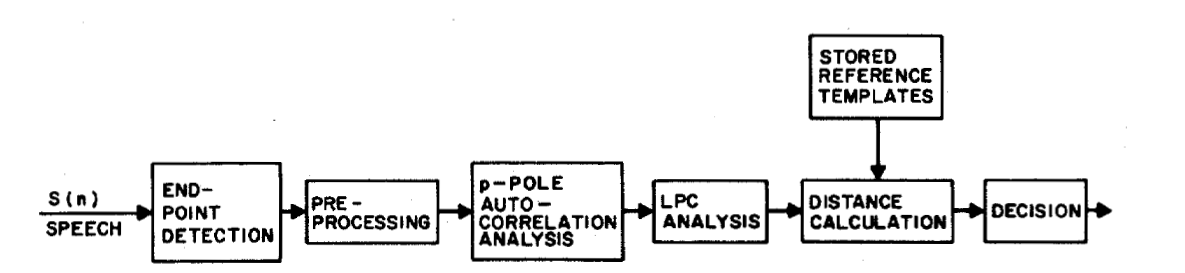
\includegraphics[width=\textwidth]{Block_digram.PNG}
\end{figure}

\end{frame}

\section{Theory and Implementation}

\subsection{Pre-Emphasis and Windowing} 

\begin{frame}{Pre-Emphasis and Windowing}
\begin{itemize}
\item Pre-Emphasis reduces the variance during distance calculation for the word recognition system
\item Filter is given by
\begin{equation}
    H(z) = 1-az^{-1}
\end{equation}
where a = 0.96 in our simulations

\item Window used is Blackman window
\item The $l^{th}$ Pre-Emphasized windowed output is given by
\begin{equation}
    x_l[n] = x[l*S + n]*w[n] \qquad 0\leq n\leq N-1, 0 \leq l \leq L-1
\end{equation}
where $S$ is the Shift, $w$ is the window, $x$ is the speech input
\end{itemize}

\end{frame}

\subsection{Feature Extraction}

\begin{frame}{Feature Extraction}
\begin{itemize}
    \item Linear Prediction Coefficients(LPC) are used as features
    \item The analysis filter is a FIR filter
    \item Predicts current value from past values
    \item A $p^{th}$ order system is given
    \begin{equation}
        \hat{s}[n] = a_1*s[n-1] + a_2*s[n-2] +\dots+ a_p*s[n-p]
    \end{equation}
    where $a_1,a_2,\dots,a_p$ are the prediction coefficients
    \item p = 8 was chosen in the simulation 
\end{itemize}
\end{frame}

\begin{frame}{LPC Extraction}
\begin{itemize}
    \item The Autocorrelation function $R(k)$ of the windowed signal is calculated
    \begin{equation}
        R(k) = \sum_{-\infty}^{+\infty} x_l[n]*x_l[n-k] \qquad 0 \leq k\leq p
    \end{equation}
    \item Toplitz Matrix is calculated
\end{itemize}

\begin{math}
\left[\begin{array}{c c c c}
R(0) &R(1) &\dots &R(p-1) \\ 
R(1) &R(2) &\dots &R(p-2) \\
\vdots &\vdots & &\vdots \\
R(p-1) &R(p-2) &\dots &R(0) 
\end{array}\right]
~
\left[\begin{array}{c}
a_1 \\ 
a_2  \\
\vdots \\
a_p 
\end{array}\right]
~ =
\left[\begin{array}{c}
R(1) \\ 
R(2)  \\
\vdots \\
a_p 
\end{array}\right]
\end{math}



\end{frame}

\subsection{Feature Matching}

\begin{frame}{Feature Matching}
\begin{itemize}
	\item Features are matched to templates
	\item The lenght of input and output need not be same
	\item Hence the Dynamic Time Warping algorithm is used
	\item If input is of length n and output of length m
\end{itemize}
\begin{align}
	D(i,j) = d(i,j) + min(D(i-1,j-1),D(i,1,j),D(i,j-1)) \\
	where \quad 0\leq i \leq n-1, 0\leq j \leq m-1 \nonumber
\end{align}
$d(i,j)$ is the distance between the feature vectors of the $i^{th}$ frame of input and $j^{th}$ frame of the template. \\
$D(i,j)$ is the Distance matrix. The final element is the DTW Distance
\end{frame}


\begin{frame}{Dynamic Time Warping(DTW)}
\begin{itemize}
	\item Greedy algorithm
	\item Warps the time scale to compensate for difference in speed and time
\end{itemize}
\begin{columns}
	\begin{column}{0.5\textwidth}
		\begin{center}
			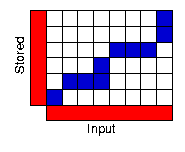
\includegraphics[width=\textwidth]{dtw.png}
		\end{center}
	\end{column}
	\begin{column}{0.5\textwidth}  %%<--- here
		\begin{center}
			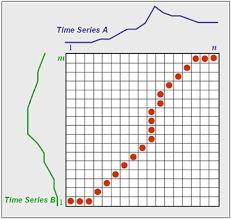
\includegraphics[width=0.8\textwidth]{dtwpic.png}
		\end{center}
	\end{column}
\end{columns}
\end{frame}

\subsection{Nearest Neighbours}
\begin{frame}{Nearest Neighbours}
\begin{itemize}
	\item The K Nearest Neighbours Rule is used for classification
	\item The KNN rule is given by
\end{itemize}
\begin{equation}
	r_j = \frac{1}{K}\sum_{k=1}^K D[x,x^{(j)}_{[k]}]
\end{equation}
\quad where $D[x,x^{(j)}_{[k]}]$ is the distance between input $x$ and $j^{th}$ word.\\ \vspace{0.5cm}
\quad $j^*$ is the recognized word, given by
\begin{equation}
	r_{j^*} \leq r_j \qquad j = 1,2,\dots,J
\end{equation}
\end{frame}

\subsection{Clustering}
\begin{frame}{Clustering}
\begin{itemize}
	\item The LPC varies from one speaker to another
	\item Large number of templates needed for better matching \\ \vspace{0.5cm}
	\textbf{But this increases computation time\\So clustering is performed} \vspace{0.2cm}
	\item In large datasets, not all speaker's LPC are distinct
	\item They can be clustered into many groups
	\item One representative is chosen from each cluster
\end{itemize}
\end{frame}

\begin{frame}{K-Mean Cluster} 
\begin{itemize}
	\item Random points are chosen as centers
	\item For each point is colsest center is chosen by distance computation 
	\item Each point is assigned to the same culster as the closest center
	\item The mean for each cluster is computed. This is the new center
	\item Steps 2, 3 and 4 are repeated for a fixed number of iteration or till error decreases below a lower bound \\ \vspace{0.5cm}
	\item An alternate version of this using the median instead of mean was also implemented
\end{itemize}
\end{frame}

\section{Simulation Results}
\begin{frame}{Simulation Results}
\begin{figure}
	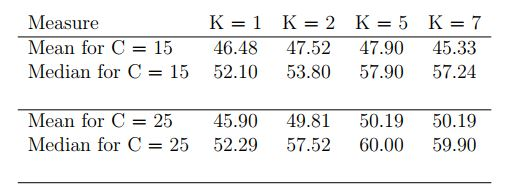
\includegraphics[width=0.7\linewidth]{result.jpg}
\end{figure}
\quad K is the number of nearest neighbours\\
\quad C is the number of cluster\\
\begin{itemize}
	\item Median clusters gave better reults
	\item K = 5 neighbours gave the highest accuracy
	\item An increse in accuracy was observed by increasing C
\end{itemize}
\end{frame}


\begin{frame}{Acknowledgements}
	\par \textit{We deeply express our gratitude towards Dr.Aparna P for giving us this wonderful opportunity to work on this project. This project gave us the opportunity to learn new and important concepts in the field of Audio and Speech Processing.}
\end{frame}

\begin{frame}
	\begin{center}
		\Huge 
		\emph{Thank You}
	\end{center}
\end{frame}
\end{document}